\documentclass[11pt]{report}



\usepackage{wrapfig, graphicx}
\usepackage[english]{babel}
\usepackage[total={5.9in,8.86in},top=1.2in, includefoot]{geometry}
\usepackage[font={small},labelfont=bf, justification=raggedright]{caption}
\usepackage{subfig}
\newcommand{\credit}[1]{\textit{(Photo: #1)}}
\setcounter{secnumdepth}{3}



\newenvironment{indpar}[1]%
{\begin{list}{}%
         {\setlength{\leftmargin}{#1}}%
         \item[]%
}
{\end{list}}



\begin{document}



\begin{titlepage}
 \begin{center}

\textsc{\large University of Toronto}\\[1.1cm]
\textsc{\normalsize AER201, January 2010}\\[1.5cm]

% Title

{ \huge \bfseries Helical Cone Deployment Machine}\\[2.4cm]

% and supervisor
\begin{minipage}{0.4\textwidth}
\begin{flushleft} \large
\emph{Group 17:}\\
Ahil Ganesh (997346466)\\
Sebastian Kosch (997241024)\\
Karl Qin (997310299)\\
\end{flushleft}
\end{minipage}
\begin{minipage}{0.4\textwidth}
\begin{flushright} \large
\emph{Supervisor:} \\
Dr. Reza Emami\\
\emph{TA:}\\
Rick Zhang\\
\end{flushright}
\end{minipage}

\vfill

% Bottom of the page
{\large \today}

\end{center}
\end{titlepage}
\setcounter{tocdepth}{2}
\tableofcontents
\chapter{Executive Summary}
The manual deployment of traffic cones, particularly on busy highways, is a dangerous and time-consuming task. The following proposal presents a prototype design for an automated traffic cone deployment machine. Automating the process is a promising way to curb accidents, speed up deployment and free up workers to do other important tasks.

The proposed design is a mobile base with a coil-based deployment mechanism not unlike those often used in vending machines. The machine is preloaded and given instructions and then operates autonomously. It can deploy cones in regular intervals as well as place extra cones on holes detected in the road surface. Upon return, the machine presents information about the deployment to the operator.

The final prototype will cost no more than \$230 CAN in materials. 

Our organizations consists of three developers: Ahil Ganesh (electromechanical design and construction), Sebastian Kosch (microcontroller programming) and Karl Qin (circuit design).

\chapter{Introduction}

\section{Statement of Need}
Traffic cones are used to create markers on roads to alert drivers and sometimes pedestrians of changing road conditions, whether this is road mergers, construction sites, potholes, or any other obstructions. Currently, traffic cones are usually deployed by hand, which is very inefficient and potentially dangerous for workers who have to work on busy streets. As such, the RFP asks for a proof of concept of a machine that can automatically deploy traffic cones on roads.
\section{Goals and Objectives}
The goal of this project is to create a working proof of concept model of a machine that can automatically deploy traffic cones in a straight line on a road. The machines should also be able to detect ``potholes'' and then cover them with traffic cones.

The machine must:

\begin{itemize}
\item{Deploy between 4 and 10 traffic cones within a designated lane 15 cm wide and 300 cm long marked by 2 lines of black hockey tape, each 2 cm wide.}
\item{Detect ``holes'' made of squares with length 5 cm and place cones on top of them; there can be up to three cones during the run. The machine must clearly signal its detection through visual or audio signals.}
\item{Deploy each cone such that the distance between its centreline and the centreline of the previous cone is within 5 cm of the instructed distance or the cone is positioned on top of a hole mark such that the mark is completely covered.}
\item{Record the location of each cone and each hole relative to the Start Line within 10 cm of real distance.}
\item{Be entirely behind the Start Line at the end of operation.}
\item{Record time of operation from when the <start> button is pushed until the machine stops and displays a termination message on the LCD. Recorded time must be within 5\% of the time measured by the referee}
\end{itemize}

The machine must also follow the following constraints:

\begin{itemize}
\item{Fit within $50\times 50\times 50$ cm\textsuperscript{3} envelope at all operation times and not exceed 10 kg in weight}
\item{Have a material cost less than \$230 CDN.}
    \item{Have its own on-board power supply.}
    \item{Be fully autonomous and does not interact with the user in any form during operation; operation commences by pressing a \textsc{Start} button on the keypad.}
    \item{Have an emergency \textsc{Stop} button that stops all mechanical moving parts of the machine.}
    \item{Can be set up and removed conveniently and without modifying the lanes.}
    \item{Display the following information at the end of each run per user's request: operation time, number of cones deployed and their distance to start line, number of holes and their distance from start line.}
    \item{Machine user interface for operation and information retrieval should be self-explanatory and simple to navigate.}
    \item{Can be set up in 3 minutes before each run.}
    \item{Can operate on hardwood or vinyl tile flooring with bright colour.}
    \item{Cannot have railway.}
    \item{Does not pose any hazard to operator.}
\end{itemize}
In addition, the machine would ideally have some or all of the following features:
\begin{itemize}
\item{Is durably constructed and functions with small failure frequency and in different conditions, including different terrains}
\item{Looks elegant and operates smoothly, with little noise or vibration}
\item{Can deploy more than 20 cones and/or work for non-straight lanes with little/no modification}
\item{Can be set up and calibrated easily in the field and all parts can be replaced/repaired easily}
\item{Fits within an envelope less than $\frac{2}{3}$ of the maximum allowed and weight less than half the maximum weight allowed}
\item{Can display date and time on LCD when in standby}
\item{Can store log information in permanent (EEPROM) memory}
\item{Can easily download operation information onto a PC}
\item{Can start and stop by remote controller}
\end{itemize}
\begin{figure}[h!]
  \centering
  \subfloat[Autocone]{\label{fig:gull}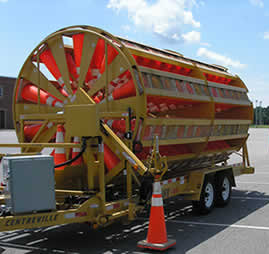
\includegraphics[width=0.45\textwidth]{autocone}}\hspace{20pt}                
  \subfloat[TRAF-tech ACM]{\label{fig:tiger}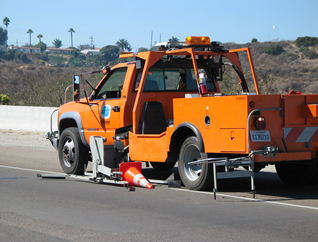
\includegraphics[width=0.45\textwidth]{traftech}}
   \caption{Existing designs \credit{http://www.innovativequip.com/, http://www.traftech.net/}}
  \label{fig:exisitingdesigns}
\end{figure}
\section{Background Research}

\subsection{Existing Designs}
\subsubsection{Autocone}
The Autocone 130 is a large trailer that stores up to 130 traffic cones. It uses a hydraulic system both to deploy the cones and to pick up cones standing or lying on the road. The cones are stored in a revolving framework. Within the framework, the cones are moved to the deployment arm by means of a chain conveyor system. While the compactness of the revolving frame is convincing, the capacity is far higher than that required in this project. For this prototype, designing an intricate miniature hydraulic arm is thus not justifiable.

\subsubsection{TRAF-tech ACT/M Series}
TRAF-tech commercialized the cone deployment system initially developed by the California Department of Transportation. Two different implementations are available: one uses rails to deploy the cones, the other a hydraulic arm. Both rely on belt systems to move the individual cones from the stack to the deployment mechanism. Like Autocone, TRAF-tech offers systems with a comparatively high cone capacity. Conveyor belts, however, are difficult to build reliably and may not be of much help with the more flexible toy cones at hand.

\subsubsection{Vending Machine Dispensing Mechanism}
\begin{wrapfigure}{r}{0.5\textwidth}
  \begin{center}
    \includegraphics[width=0.48\textwidth]{vendingmachine.jpg}
  \end{center}
  \caption{Coil-based vending machine}
\end{wrapfigure}


Many common vending machines that dispense bags of chips or candy bars employ a coil mechanism for dispensing merchandise. Most modern vending machines employ the use of a motor that spins a metal coil dispenser. The packages are placed in between each ridge of the coil. As the motor turns the packages are pushed forward and when a package reaches the front of the coils it falls out due to gravity and is ready for the customer. 
In this project, a simple method for dispensing cones is required. As stated before hydraulic arms and conveyer belts prove to have many limitations and are not justifiable. This coil system though provides a simple method of keeping the cones separate and require the use only a few moving components.


\chapter{Conceptualization}
\section{Dispensing Mechanisms}
\begin{figure}
  \centering
  \subfloat[Fork]{\label{fig:fork_system}\includegraphics[width=0.46\textwidth]{fork.jpg}}  
\hspace{20pt}             
  \subfloat[Conveyor Belt]{\label{fig:conveyorbelt_system}\includegraphics[width=0.46\textwidth]{conveyor.jpg}}
  \caption{Dispensing Mechanisms}
  \label{fig:dispensing_mechanisms}
\end{figure}

During our initial brainstorming a number of possible dispensing mechanisms were discuss. Below are outlined discussed mechanisms involved in dispensing the cone as well as some limitations of each possible design.

\paragraph{Fork System}
In this system, a fork-like system pulls the bottom cone off that stack of cones. Two prongs form each side are separated by a distance such that only one cone base will fit in between. The prongs would extend from the sides of the stack and slide into the bottom cone's base. The prongs would pull the bottom come down and then retract allowing the bottom cone to drop. Lever-and-pivot systems may be the easiest to implement, since they only require actuation in two directions.

\begin{indpar}{1cm}
Limitations of this design: Since the cones are made of a rubber material, it is highly likely that the cone bases would be bent in some form. The bending of the cone's base would make the precision of the prongs to grasp the bottom cone's base extremely important. The timing of the retraction of the forks would also need to be very precise. In addition, further support would be required to hold the remainder of the stack in place while the bottom cone falls.
\end{indpar}

\paragraph{Conveyer Belt System}
In this system, the cones are separated and move along a conveyer belt system. When they reach the end of the conveyer belt, the cones would be pushed off, while the next cone moved into place.

\begin{indpar}{1cm}
Limitations of this design:
Space usage in this design is very large since the cones would not be stacked. In addition, conveyer belts require high tension in order to work effectively, this would be quite difficult to maintain.
\end{indpar}

\paragraph{Stacked Conveyer Belt System}
This system is a combination of the previous two. Two gear and chain systems would be present on each side of the stack of cones. Along the chain there would be protrusions that would be able to separate the cones in the stack. The chain would rotate downward and then cones would move down. When a cone got to the bottom the protrusion holding it would turn downward and the cone would fall while the others cones are held in place by the individual protrusions.

\begin{indpar}{1cm}
Limitation of this design:
There are number of moving parts in this system that would be prone to failure. Fabricating the required gear and chain would require very specific materials and would be likely to break.
\end{indpar}

\paragraph{Claw System}
In this system, the cones would be stacked and a claw would come down and lift off the top cone. The claw would have a similar prong system to that in the Fork System for separating the top cone from the rest of the stack.

\begin{indpar}{1cm}
Limitations of this design:
A claw system requires a large number of moving parts which would be prone to error and malfunction.
\end{indpar}

\paragraph{Coil System}
This system is similar to a vending machine chip dispenser, in which a coil rotates moving the stack of cones to the bottom. When a cone reaches the bottom of the coil, it falls off the stack. This method ensures that the cones remain separated by a distance that would allow them to be easily detached from the stack when they are dropped.

\begin{indpar}{1cm}
Limitations of this design:
In this design the initial loading of the cones is the main limitation. Cone would either need to be loaded in one by one while the coil turns one turn in the opposite direction or would need to be loaded in at the same making sure that each cone is separated in the spring by the correct number of turns.
\end{indpar}

Below is a Pugh chart that was used to compare the above possible designs. We can see that the coil system received the highest score when compared to what we consider the most important requirements for the cone deployment system. Although the claw system would be very accurate in the deployment of the cones, it would require many moving parts that increase the complexity of the machine.
\begin{figure}[h!]
  \begin{center}
    \includegraphics[width=\textwidth]{ConePugh}
  \end{center}
  \caption{Comparison between dispensing mechanisms}
\end{figure}



\section{Circuit subsystem}


%%%%%%%%%%%%%%%%%%%%%%%%%%%%%%%%%%%%%%%%
% Karls stuff
%%%%%%%%%%%%%%%%%%%%%%%%%%%%%%%%%%%%%%%%



\subsubsection{Hockey Tape Sensors}

The main sensory requirement of this project is sensing black hockey tape on the ground. The robot will need to follow a designated lane created by parallel hockey tapes and detect holes on the ground, also created by black hockey tape.

The main difference between the floor and the markings will be colour. This gave rise to two possible solutions to the sensor problem:
\begin{itemize}

\item{\textbf{IR Photoreflector:}
IR photoreflectors usually come as a unit, housing a LED and a phototransistor. The LED emits infrared radiation, which than hit the surface. Depending on the color (in the IR spectrum) of the surface, IR will be reflected and hit the phototransistor. The voltage loss across the phototransistor will change depending on the amount of light hitting it. In this way, The IR photoreflector can detect different colours. }

\item{\textbf{Color Sensor:}
An alternative to the IR photoreflector is the color sensor. It operates on the same principles, except the LED now emit in the visible light spectrum and the photoelectric receiver is either a photoresistor or a photoiode that can detect a specific wavelength (and therefore colour) of visible light.}
\end{itemize}

Since infrared radiation is used instead of visible light, it cannot differentiate between many colours of the visible light spectrum. For the purpose of this project, however, there will only be two different surfaces: the light coloured floor and the black hockey tape. Given that black objects absorb IR much more readily than light coloured objects, IR photoreflectors should suffice in for this project. The TCRT5000L optosensor was tested and found to have an effective range of around 1.5$\pm$0.5cm, which will be enough for this machine as it will operate on smooth ground and can leave sensors very close to the floor. If this is not enough, the TCND5000 photoreflector from the same manufacturer (Vishay) has a maximum range of 40mm and should suffice for this purpose.

Colour sensors are much more advanced: they can detect specific colours and works on a narrower spectrum; so they will be more precise in detecting the hockey tape (which will absorb all visible light). However, they are more expensive than the IR photoreflector. Therefore, colour sensors will not be used unless further trials of the IR photoreflectors reveal unexpected problems.

\subsubsection{Additional Sensors}

Two additional sensory requirements are shaft encoders and traffic cone detection

\paragraph{Shaft encoders}
To figure out the distance travelled, the machine will use shaft encoders to determine the number of rotations that the wheel has taken. Shaft encoders are essentially photoreflectors paired with a circular dark and light pattern mounted onto the axel. As the wheel spins, the photoreflector will hit dark and light spots of the pattern in a regular fashion and produce a wave pulse. A certain number of wave pulses will then indicate that the wheel has come full circle. Given the circumference of the wheel, the machine’s microcontroller can then determine the distance travelled by the machine. 
\newline\newline
As in the case of the hockey tape, an IR photoreflector will be used. Alternatively, the machine can use a break beam sensor in conjunction with a plate that has alternating notches in it that will block the emitted light in a regular pattern. If not possible, the distance can also be crudely measured by calculating the amount of time the motor was powered and pre-configuring the speed of the wheels.

\paragraph{Traffic Cone Detection}
In the proposed design, there is no simple method of detecting whether the machine is empty of traffic cones or not. Given that the user cannot input the number of traffic cones into the machine, there must be a sensor to detect the presence of cones. There are three prposed methods of cone detection:
\begin{itemize}
\item{\textbf{IR Photoreflector:}
The photoreflector was accurate for hockey tape detection because it was possible for the photoreflector to be placed very close to the smooth ground. However, in this situation, there is a shaft around the traffic cones that prevents the sensors from being placed too close. Thus, the cones may be out of maximum range.}
\item{\textbf{Color Sensor:}
Similar to the photoreflector, the color sensor has a very limited range and may not be suitable for these uses. However, its ability to see the “orange” light should be an asset in this use.}
\item{\textbf{Break Beam Sensor:}
An LED emits IR light from one side of the cone compartment, while a phototransistor sits on the other side, directly opposite. While cones are present, the phototransistor detects nothing, and when the machine is empty, the light emitted from the LED can then be detected. }
\item{\textbf{Ultrasonic Proximity Sensor (Sonaswitch Mini S):}
This sensor works very much like photoreflectors, except instead of using light, it emits ultrasound and receives the echo, which will differ depending on the presence or absence of traffic cones. It is accurate and can work for great distances, however, it is very expensive (\$10 at the design store) and much larger than the other sensors under consideration.}
\end{itemize}

The break beam sensor promises to be very accurate, but it must be mounted on two opposing sides of the cone dispensing mechanism. This may be very difficult in the proposed design; so a mechanism that transmits and receives from the same side is preferred. The ultrasonic proximity sensor is also under consideration because it has a greater range. However, it is relatively expensive and very bulky to mount.

If possible, the machine will use an IR photoreflector to detect the cones; if it becomes apparent that they do not have the range necessary to perform this task, the machine will use an ultrasonic proximity sensor.

The Pugh Chart below shows the evaluation of the 4 different types of sensors.

\begin{figure}[h!]
  \begin{center}
    \includegraphics[width=\textwidth]{SensorPugh.JPG}
  \end{center}
  \caption{Comparison between different types of sensors}
\end{figure}

\subsubsection{Motors}

Two tasks require motors in this project: moving the machine and dispensing the traffic cones. Therefore, three types of motors are considered for this project:
\paragraph{DC Brush Motor}
DC motor is the simplest motor to control both in terms of speed and in terms of direction. It also has a high torque to weight and torque to cost ratio, making it a very economical choice. However, its rotation cannot be controlled accurately.
\paragraph{Unipolar Stepper Motor}
The unipolar stepper motor moves the rotor a certain number of degrees after receiving a series of pulses from the controller through a series of wires. This gives the user a large degree of control over the rotation of the motor. The control circuit for the stepper motor is quite complicated (though there are readily available stepper driver IC’s like the ULN2001A that make this much easier). 
\paragraph{Servo Motor}
A servo motor is a powerful motor that uses a feedback mechanism to control the position of the rotor, it is very useful when the machine needs the rotor to hold at a certain position. It also has a high torque. However, the servo motor is very complex and may not be able to rotate fully (i.e. 360 degrees).
\newline\newline
The wheels of the machine will be powered by DC motors due to their simplicity and versatility. The stepper motor is too weak to move the entire machine, and the servo motor is restricted in its movement. The wheels of the machine do not have to turn very precisely and requires a high torque, thus the DC motor is the obvious choice.

The dispensing mechanism will use a stepper motor because every full rotation will release a traffic cone. If the rotation is off, or there is error in the rotation, the traffic cone may not deploy or multiple cones may deploy at the same time. Therefore, a high degree of control is required, thus ruling out the DC motor. Furthermore, the mechanism needs to make full revolutions, but high torque is not necessary, so a servo motor would not be useful in this machine. A stepper motor is very precise and will allow the machine to dispense exactly one traffic cone at a time, so it is the obvious choice.



\chapter{Technical Body}
\section{Components}

\subsection{Electromechanical Subsystem}
This machine is designed to travel along a lane and dispense traffic cones at specified lengths or upon detection of a hole. As the machine moves forward, a cone will be dispensed from the back of the machine and fall in place at the specified length. 

The dispensing mechanism is a coil system in which the cones are placed in the ridges of a metal coil. As the coils turn, the stack of cones moves downward until the bottom cone is dropped out of the coils. This method of dispensing is commonly used in vending machines. 

The machine will be propelled by four wheels. The two front wheels will be connected to two individual motors and the rear wheels will be free to follow the movements of the front. The use of two motors will facilitate the steering required for the machine to stay within the designated lane.

This machine will have dimensions of $47\times 26\times 30$ cm\textsuperscript{3}.

\paragraph{Wheel System}

This machine will employ a two wheel drive system. The two front wheels will each be connected to a Shenzhen DC gearhead motor. The wheels themselves will be fixed parallel to the body of the machine. None of the four wheels will have steering mechanisms. Each wheel will have its own axel and will not be connected to the other wheels in any way.

The shaft of the motors will be inserted into another larger shaft, which will be fabricated using an aluminum rod, and will be held in place by a locking screw. The wheel will then be placed directly onto the shaft and bolted in place. 

The individual motors for the two front wheels allow for steering to be controlled by the speed of the motors. When the machine needs to turn in a specific direction, the opposite wheel will turn faster as controlled by the motor. 

\begin{figure}
  \centering
  \subfloat[Wheels]{\label{fig:fork_system}\includegraphics[width=0.3\textwidth]{Wheels}}  
\hspace{20pt}             
  \subfloat[Coils and Cones]{\label{coilsCones}\includegraphics[width=0.3\textwidth]{ConeCoil}}
  \caption{Mechanical Components}
\end{figure}

\paragraph{Coil System}

In order to store and dispense the traffic cones, two steel coils will be used similar to those used in snack vending machines. Each coil will be attached to a wooden cylinder using brackets. A screw will be inserted through the wooden cylinder and then inserted through a wooden support beam from which the coils will hang. A gear will then be placed tightly onto the screw and secured with a bolt. Ball bearings will be placed between the gear and the wooden support plank to reduce friction during rotation. Two of these coil mechanisms will be used to support both sides of the cones.  

A universal stepper motor will be used to turn both of the coils. The motor will be connected to a gear using a shaft fabricated from an aluminum rod. A locking screw will be inserted into the side of the motor to keep the fabricated shaft connected to the shaft of the motor. The rod will then be placed through a gear and then bolted securely to the wooden support plank. 

The bottoms of the coils will also have a support system to prevent them from moving apart during operation of the machine and causing the cones to fall out. Half of a wooden cylinder will be secured to a wooden plank. The half cylinder will be placed inside the coils as shown in the figure \ref{coilsCones}. The wooden plank will have a groove at the base of the half cylinder for the coil to follow as it turns. The wooden planks will be attached to the frame of the machine.

The sides of the cones that are not supported by the coils will be supported by a plexiglass wall. This will provide stabilization for the cones and ensure that they fall perpendicular to the floor.

During operation, the cones will be stacked and each cone will be separated by a single ridge of the coil, as shown in the figure \ref{coilsCones}. As the motor turns, the gear system causes the two coils to turn in unison. As the coil turns in a clockwise direction, the cones move down the coil. When a cone reaches the bottom of the coil it will fall out while the rest of the stack remains in place in the coil. As the cone falls the support walls will help it to remain upright and land correctly on the floor.


\paragraph{Frame and Casing}
The frame of the machine will be fabricated using aluminum angles which will be screwed together in the shape of the frame. For sketches of frame see appendix C. Plexiglass will then be used to fabricate the walls of the machine. The plexiglass will be cut down to size and then glued to the metal frame. A door will be present in the plexiglass for loading of the cones. The cones will all be stacked and loaded simultaneously into the coil system. The coil system will be located in the rear half of the body of the machine. The front half of the machine will house the boards and the main circuitry. 

\paragraph{Material Selection}

As stated before, the frame itself will be fabricated using aluminum angles. This choice of materials provides a stable frame while still being lightweight. The walls of the machine will be fabricated using plexiglass. Like the aluminum, plexiglass provides a durable yet lightweight option. The interior of the machine will have a wooden plank as a bracket to hold and support the coil system. Wood was chosen due to the weight of the coil system. If plexiglass were to be used, the weight of the coil system would cause the plexiglass to deflect and bend under the weight of the coils.

For the coil system, two metal coils will be used. Although metal is a heavier material, its strength and high yield provide a durable option. A wooden dowel will be used to secure the coils to the gear system. The wood provides facile means of securing the coils. Plastic gears will be used in this machine for the gear mechanism, as metal gears have a high weight associated with them.



\subsection{Circuit Subsystem}
\begin{wrapfigure}{r}{0.5\textwidth}
  \begin{center}
    \includegraphics[width=0.48\textwidth]{sensors}
  \end{center}
  \caption{Photoreflector Circuit}
  \label{SensorDiagram}
\end{wrapfigure}

\paragraph{Sensors Overview}

All sensors used in this machine will be IR optosensors (TCRT5000L/ TCND5000), if they are found to be inadequate, they will be upgraded for better range and capabilities at the discretion of the team following the guidelines laid out in survey.

The circuits for these sensors are very simple. The LED simply needs to be powered by a 5V power supply with an appropriate resistor to reduce the current. The phototransistor will similarly be connected to the power supply and a resistor. As IR light hits the phototransistor, the voltage gain across it will change. (See figure \ref{SensorDiagram})

The voltage can then be sent to the microcontroller (after the current has be sufficiently reduced) to be converted into a digital signal.




\paragraph{Sensor Allocation}
There will be 10 sensors in 4 different roles in this project that will feed information to the microcontroller that controls the circuit.
\begin{itemize}
\item{\textbf{Lane Sensing (4):}
There will be 2 sensors beside each wheel to see whether the machine is straying off the lane. In normal operation, both sensors will be over bright vinyl and will thus record similar voltage outputs. Once one of the sensors crosses onto the black line, there will be a great voltage difference between the two and the microcontroller will know to correct the course of the machine. This configuration will, to a great extent, remove the influence of ambient lighting on the results of the sensors.}
\item{\textbf{Hole/Start/End Sensing (3):}
There will be 3 sensors placed in an array across the front of the machine spaced 2cm apart. At 0m and 3m, they will search for start and end lines. In between, however, the machine will search for “holes”, and once it has found one, the sensors’ output voltage will change and notify the microcontroller to commence cone deployment. The 3 sensors across 6cm will compensate for any deviation of the holes or the machine from the centerline.}

\item{\textbf{Shaft Encoding (2):}
Two IR sensors will be placed beside the shafts so that they can sight circular disks on the axles that will spin with the wheels to notify the microcontroller how far they have travelled. As the wheel spins and the sensor sees dark or light patches, its output voltage will change constantly. By counting the wave pulses (after being processed by an analog to digital converter), the microcontroller will be able to know the exact distance travelled by the machine.}
\item{\textbf{Cone detection (1):}
For cone detection, a TCRT5000L or TCND5000 will be placed at the base of shaft. After the machine begins operation, the sensor should have a certain voltage output, when the shaft is completely empty, the sensor will have a completely different voltage output. The microcontroller will check this sensor reading after every single deployment. If the sensor’s reading has changed dramatically, the microcontroller will cease operation and turn around.}
\end{itemize}



\paragraph{Motors}
There are two different types of motors used in this machine, DC and stepper. Two DC motors drive in differential drive the wheels and the stepper motor drive the deployment mechanism.
\begin{figure}[h!]
  \centering
  \subfloat[DC Motor]{\label{dcmotor}\includegraphics[width=0.3\textwidth]{dc}}  
\hspace{20pt}             
  \subfloat[Stepper Motor]{\label{steppermotor}\includegraphics[width=0.3\textwidth]{stepper}}
  \caption{Motor circuit diagrams}
\end{figure}
\begin{itemize}
\item{\textbf{DC Motor:}
The DC motor needs to be powered and its speed must be controlled. Given the design of this machine, it will not need to reverse direction (it will instead turn around to go back to the starting line). The DC motor needs a 12V power supply to run. It will be controlled by Pulse Width Modulation sent out by the microcontroller, which can then control an NPN transistor that will then power the circuit. Note that no H-bridge is needed because the car will turn to return to start line, the wheels will thus not need to reverse direction. (See \ref{dcmotor})}
\item{\textbf{Stepper Motor Circuit:}
The speed of the stepper motor will also be controlled by pulse width modulation sent out from the microcontroller. The signal will pass to the ULN2001A stepper motor driver IC before being sent to the stepper motor itself. H-Bridge is not necessary as the motor will only turn in one direction and the motor used will be unipolar. See \ref{steppermotor})}
\end{itemize}
\paragraph{Signal Protection/Condition}
At this early stage, it is still uncertain how the circuits will interact/interfere. However, it is certain that every circuit containing logic chips will require protection from surges and the noise in any signal going from the sensor to the PIC and any signal going from the PIC to the motors will need to be filtered. While it is too early to accurately describe the circuits, this proposal will make some worst case scenario estimates on the diodes, op amps, conductors, and inductors needed in this project.


\paragraph{Power Supply}
The machine will be powered by a number of D cells. They have the advantage of being powerful enough to power the motors in the circuit while still being modular. At this early stage, without torque or weight calculations, it is impossible to calculate the power needed. Therefore, using a number of D cells placed either in parallel or series will allow the exact power supply configuration to change after more tests and calculations have been done.

The motors and the other electronic components will be powered by separate groups of D cells. This is because the motors require a large current, and by isolating them, it prevents accidental surges on the logic chips.

The emergency switch for this machine will be placed right between the power supply and the motors. This will allow the rest of the machine to continue to operate and provide information to the user even as the mechanical parts come to a complete stop.


\subsection{Microcontroller}
A single microcontroller processes the sensors' inputs, computes the power delivered to the motors, and interacts with the user via a matrix keypad and a 16$\times$2 character LCD. 
\paragraph{Choice of model}
The microcontroller used is a 40-pin PIC chip by Microchip, model 18F4620. The model was chosen over model 16F877, which was given with the development board, mainly for its interrupt capabilities. The 16F series provides an external interrupt channel on pin \texttt{RB0}. Unfortunately, this does not allow for interrupt-based development with the development board's keypad, since the keypad's \texttt{DataReady}-flag is hardwired to \texttt{RB1}. Using the Interrupt-on-change feature on \texttt{RB4:7} does not help; pressing the same key twice will not raise an interrupt. The same rationale explains the choice of a 40-pin model. While all functionality could have been implemented, tested and debugged on the development board with the given 16F877 series PIC, interrupt-based code is easier to debug than code littered with \texttt{goto}-based polling points.  

\paragraph{Program flow and menu}
On power-on, the microcontroller initializes memory, interrupt bits and I/O settings. It then waits for input on interrupt lines, and potentially enters a power-saving mode to reduce battery strain. The following events should raise an interrupt:
\begin{itemize}
  \item{the user presses a key on the keypad,}
  \item{the interval timer overflows to cause a cone to be deployed,}
  \item{the reflection sensor reports a hole,}
  \item{all cones have been deployed, or a distance of 3 meters was covered,}
  \item{the side reflection sensors report crossing the lane.}
\end{itemize}
\begin{figure}
  \centering
  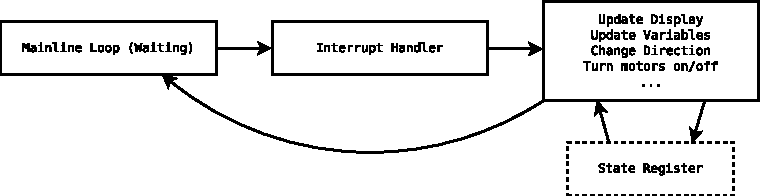
\includegraphics{program_flow.pdf}
  \caption{General flow of the microcontroller program}
  \label{fig:programflow}
\end{figure}
The interrupt service routine (ISR) will then determine the type of interrupt. A state register holds a numerical value representing the current state of the device, such as \textit{Menu, Screen 3} or \textit{Returning from deployment}. Depending on the current state, the ISR calls subroutines to handle the input. Example: during user interaction, this might mean storing the input and updating the display; during deployment, this might mean rotating the coil or decelerating the motors. It may also include changing the state register. Eventually, all subroutines will return to the \texttt{Mainline} loop to save power.

The menu (already successfully implemented at this point) functions as follows: 

\begin{verbatim}
Interrupt:
select state		;holds the number of the current screen or operational phase
case 1		;Welcome screen
select key\_pressed	;from RB4:7
case D
call menu\_next
endcase
endselect

case 2		;Options screen
.
.
.

menu\_next:
state++
call menu\_drawscreen
.
.
.

menu\_drawscreen:
select state
case 1
print ``Welcome    ''
print ``    Start:D''
.
.
.
\end{verbatim}

The interrupt triggered by pressing a key on the keypad is evaluated against the current value of {\tt state}, the register that holds the number of the current screen, or otherwise operational phase. Depending on the pressed key the {\tt state} register's content is changed, values are entered (for example, when the user enters the time or a deployment interval), or nothing happens. Eventually, {\tt menu\_drawscreen} is called. This routine draws the available data on the screen, depending on state and the user's input.

User input of numbers requires special attention: the entered bits have to be converted to a numerical value, and this numerical value has to be represented as a digit on the screen right away, in the proper position. How this is done depends on the register {\tt parammode}. Here an example of how the user input is handled when in the third screen (entering the offset from the start line):

\begin{verbatim}
Interrupt:
...
case 3
select key_pressed
case 0-9
call param_append
case C
call param_delete
case D
call menu_next
endcase
.
.
.

param_append:
digit3 = digit2
digit2 = digit1
digit1 = key_pressed
call menu_drawscreen

param_delete:
digit1 = digit2
digit2 = digit3
digit3 = 0
call menu_drawscreen

menu_drawscreen:
...
if(parammode = 1)
set_LCD_cursor_to(7)
print digit3
print digit2
print digit1

param_offset = 100*digit3 + 10*digit2 + digit1
\end{verbatim}


Using this Binary-coded decimal representation, entered digits are easily processed and quickly converted into the actual value (using PIC18's hardware multiplier). Once deployment starts, data must be collected for future reference. The data collected during one deployment (``data set'') is structured as follows:

\begin{enumerate}
\item{timestamp (3 bytes)}
\item{cone\_positions (10*2 bytes)}
\item{cone\_types (2 bytes)}
\item{dist\_traveled (2 bytes)}
\item{cones\_deployed (1 byte)}
\end{enumerate}

Before deployment, all these registers are cleared, and the FSR registers are set to the addresses of cone\_positions, cone\_types and dist\_travelled, so that these arrays of values can easily be filled with data during deployment.

If the user chooses to save and view the data after deployment, the data set is appended to the PICs nonvolatile EEPROM for future access. The data view window is then shown, and the last data set can be browsed. Similarly, the data view window accessible via the Options window (screen 2) allows access to all past data sets, and provides a means to erase all data on the EEPROM. The following structure controls the machine's operation during the deployment stage. Interrupts, triggered by overflowing timers and changing outputs from the sensors, cause the deployment of cones or a turning maneuver.

\begin{verbatim}
Begin_deployment:
Lfsr	0, cone_positions
Lfsr	1, distance_traveled
Lfsr	2, cone_types

Timestamp = current_time

; Timer1, Timer2, LaneSensor, HoleSensor cause ...

Interrupt:
Select Interrupt_type
Case Timer1			;distance/cones_remaining
	;check if we're past 3 meters, or if we're out of cones
	;if yes, goto return_home

Case Timer2			;offset/interval
	;check if it's time to drop a cone
	;if offset=1, set offset=0 and interval=param_interval
	;if yes, goto deploy_cone

Case LaneSensor
	;if too far left, increase left motor speed
	;if too far right, increase right motor speed
	;if on track, go back to equal (regular) motor speed
	
Case HoleSensor
	;if detected a hole, goto deploy_cone



Deploy_cone:
	;turn on stepper motor PWM
	;wait for X cycles, corresponding to 360 degrees
	
	W=2
	Cones_deployed++
	PLUSW0 = currentDistance	;write current distance into one_positions
	INDF2.pin(cones_deployed) = currentHoleType	;record the type of hole deployed

Return_home:
	;turn on right motor, turn of left motor
	;wait for Y cycles (experimentally determined)
	;turn on both motors, full speed
	;go back by INDF1 (distance_travelled) plus 20cm to be sure
	;display success screen
\end{verbatim}



\subsection{Functional Description}
The cone deployment machine will prompt the user for input, deploy the cones, return to the user and display information about the deployment. This communication happens via a 4$\times$4 matrix keypad (keys 0--9 and A--D) and a 16$\times$2 character LCD with standard HD44780 interface. To make operation as easy as possible, the interaction using display and keypad should be self-explanatory to the user. Therefore, we designed a near-linear sequence of inputs and outputs that leads the user through all necessary steps. This is adequate for both novices and experiences users. Figure \ref{fig:menuflow} provides an overview.
 
As the user interacts with the machine through the LCD and the matrix keypad, the user will be prompted to place the cone into the machine by liftiing up the back wall of the cone shaft and inserting the cones. After pressing the <start> button, the machine will operate on its own. It will first sense the start line via its frontal sensors and alert the PIC to commence regular operation, after which the machine will place a traffic cone after a distance preset by the user. Subsequently, the machine will place traffic cones at regular intervals, in both cases, the distance information will be collected by the shaft. After a hole is detected by the frontal sensors, the PIC will send a series of pulses to the stepper motors to dispense a cone. At 3 m (as determined by the shaft encoders) and/or when the machine detects the end line (when the machine detects the fourth "hole"), the machine will turn around by pivoting on one of its wheels by having the microcontroller open the switch to one DC motor while simultaneously closing the switch to the other). The number of revolutions needed to complete the turn will be determined by the circumference of the wheel and the distance between the two wheels, the machine will accomplish this turning action by sending a preset number of wave pulses to one of the DC motors.
 
Finally, after an entire operation, the machine will return to the user behind the start line (as determined by the shaft encoder and/or the machine detects te beginning line in a similar manner to above) and yield all of the data gathered by the machine and stored onto the PIC during its operation.


\subsection{Evaluation Plan}
\subsubsection{Process evaluation}
Process evaluations are an important activity for keeping the team on time and budget and evaluating the progress of the project. Important milestones and timelines for various tasks have been outlined in the Gantt charts in the appendix. These timelines are important as they keep the group on track towards successful completion of the project. Members should plan each week so that all required tasks are completed.

Group meeting also provide an important opportunity for process evaluation. During meetings, the entire group will be able to examine the progress of not only themselves but also other group members. During these meetings, group members should remind themselves of key deadlines and upcoming tasks. They should also examine the budget and discuss important purchases that have and will need to be made. Members should note that although they are working independently on their subsystem, they should consult the team about design decisions and concerns.
\subsubsection{Product evaluation}

Project evaluations are an important method of monitoring the progress towards the final product. The purpose of these evaluations will be to test fabricated components to ensure functionality. During the first half of this project, the individual members will test their respective subsystems. After the completion of each major component thorough testing should be completed in order to ensure that there are not any flaws. Debugging of the individual subsystem components will aid in the integration of the subsystems in the second half of the project. 

At the time of integration, testing becomes a very important aspect; a large amount of time has been allocated towards testing and troubleshooting. After the completion of each major integrated component, thorough testing should be completed to ensure the required functionality. Further testing should be completed once all components have been integrated. 

\section{Schedule}
\newpage
\section{Budget}
\begin{figure}[h!]
  \begin{center}
    \includegraphics[width=\textwidth]{Budget.JPG}
  \end{center}
  
\end{figure}
\chapter{Conclusion}
The proposed design’s greatest appeal like in its simplicity as the number of moving parts has been reduced to the motors driving the wheels and the coils. It simply required two motor driven coils which will rotate and drop a one cone at a time. No clamping or pulling mechanisms are required. The greatest challenge in this project will be to ensure that the coil system functions properly. It requires a great deal of calibration and synchronisation, and if unsuccessful, will set this project back a great deal and require the alternatives to be reconsidered. However, extensive prototyping has proven that the theoretical concept is sound and that this is a viable method.

The greatest challenge will be ensuring accuracy, but experiments with retractable side walls have been successful in helping to facilitate accurate deployment of cones. The most crucial and rate-limiting step is the coil mechanism. Care and perfection will allow for this mechanism to deploy a single cone from the stack at the required length.

If successful, this mechanism will prove to be easily translated into a life size prototype, as a car that can be towed behind a trailer.

\appendix
\chapter{Appendix}
\section{Bibliography and References}

[1] United States Department of Transportation. (2010). Frequently Asked Questions -Part 6 - Temporary Traffic Controls [Online]. Available: http://mutcd.fhwa.dot.gov/knowledge/ faqs/faq\_part6.htm
\newline\newline
Levasseu, Joseph (2007).Patent No. 0199951. USA. Accessed January 24, 2011.
\newline\\
HowStuffWorks Express. (2008). HowStuffWorks Autopsy: Inside a Vending Machine [Online]. Available: http://express.howstuffworks.com/autopsy-vending.htm
\\\\
Innovative Equipment. (2011). Autocone 130[Online]. Avalable: http://www.innovativequip.com/
\\\\
Traf-Tech. (2011). Cone Trucs [Online]. Available: http://www.traftech.net/

\newpage
\section{Figures and Tables}
\begin{figure}
  \centering
  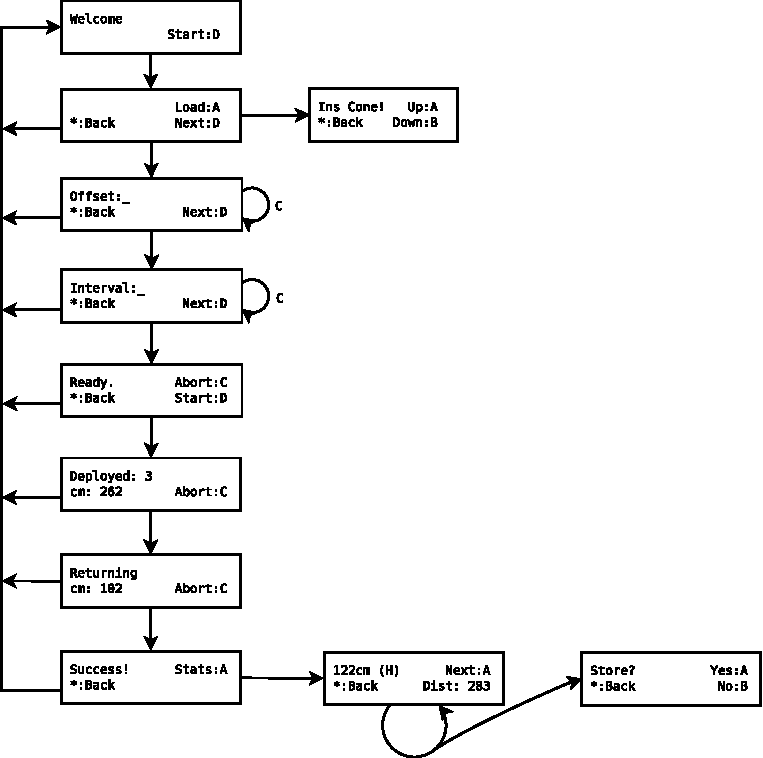
\includegraphics[width=\textwidth]{menu_flowchart.pdf}
  \caption{Sequence of menu displays navigable by the user}
  \label{fig:menuflow}
\end{figure}
\begin{figure}
  \centering
  \includegraphics[width=\textwidth]{insert_view}
  \caption{Inserting the cones into the machine}
  \label{fig:menuflow}
\end{figure}
\begin{figure}
  \centering
  \includegraphics[width=\textwidth]{front_view}
  \caption{Front view}
  \label{fig:menuflow}
\end{figure}
\begin{figure}
  \centering
  \includegraphics[width=\textwidth]{side_view}
  \caption{Side view}
  \label{fig:menuflow}
\end{figure}
\begin{figure}
  \centering
  \includegraphics[width=\textwidth]{top_view}
  \caption{Bird's eye view}
  \label{fig:menuflow}
\end{figure}
\begin{figure}
  \centering
  \includegraphics[width=\textwidth]{back_view}
  \caption{Back view}
  \label{fig:menuflow}
\end{figure}
\newpage
\section{Evidence of Capability}
We believe that evidence supports our team's capabilities:
\begin{itemize}
\item {A prototype of the deployment mechanism was developed and tested in less than a week after receiving the RFP; the preliminary main components of the mechanism were finished during the second lab.}
\item {The entire PIC program was outlined within days after receiving the development board. During two days of programming, half of the menu and data structures were successfully implemented and tested and presented during the second lab. We expect the remaining functionality to be implemented within another weekend, such that more manpower can be devoted to the physical construction.}
%\item {Our microcontroller member, who has himself taught programming classes for several years, is using a custom programming environment and a distributed versioning system to have fine control about the workflow.}
\end{itemize}
%\bibliography{


%}

\end{document}
